	% Template for a challenge (and solution) for the MATH+ advent calendar.
	
	% Please save the document as follows:
	% MK-2020-Authors-ShortTitle-en.tex

\documentclass[12pt]{article}
\usepackage{amsmath}
\usepackage{mathtools}
\usepackage{amssymb}
%\usepackage{dsfont}
\usepackage{graphicx}
\usepackage{pgf,tikz}
\usetikzlibrary{shapes.geometric,calc}
\usetikzlibrary{arrows}
%\usepackage[ngerman]{babel}
%\usepackage[utf8]{inputenc}

	% Please insert additional LaTeX packages needed!

%%%%%%%%%%%%%%%%%%%%%%%%%%%%%%%%%%%%%%%%
%%%%%%%%%%%%%%%%%%%%%%%%%%%%%%%%%%%%%%%%

\setlength{\parindent}{0cm}

\begin{document}

	% Please insert the title of your challenge, the name(s) of the author(s), and you project title!

%\setcounter{section}{0}

\section{Water Supply Network}

Authors: Axel Kr\"oner (WIAS), Hong Nguyen (WIAS)

\subsection{Challenge}
Far away in Frozen Kingdom, to guarantee a happy Christmas holiday, Santa Claus and some elves Alice, Bob, Camille, Dominic, Elsa, Federico, and Gwen want to set up a water network to supply water to watermills in order to make flour for cookies. Precisely, $m$ water supply factories denoted by $(F_i)_{i=1}^m$ will supply $n$ watermills $(W_j)_{j=1}^n$. For each $i = 1,\dots,m$ and $j = 1,\ldots,n$, the factory $F_i$ stores water of volume $V_i$ in its own water tank and is connected to the watermill $W_j$ by an individual empty pipe, denoted by $p_{ij}$, being uniformly cylindrical with the size uniquely characterized by a fixed wall thickness $\delta > 0$, length $l_{ij}$ and radius $r_{ij}$ of its interior. At the inlet of each pipe $p_{ij}$, a water pump engine is configured to supply water with a constant \emph{volumetric flow rate}\footnote{\textit{Volumetric flow rate} of water is defined to be the volume of fluid $V$ which passes during a period of time $t$: $Q \coloneqq \frac{V}{t}$.} $Q_{ij}$ (in $\rm m^3/s$).

\begin{table}[h]
    \centering
    \begin{tabular}{|c|l|}
        \hline
        \textbf{Notation} & \textbf{Meaning} \\
        \hline
        $p_{ij}$ & the uniformly cylindrical straight pipe connecting $F_i$ with $W_j$ \\
        \hline
        $\delta$ & thickness of each pipe in the network. \\
        \hline
        $l_{ij}$ & length of the pipe $p_{ij}$ \\
        \hline
        $r_{ij}$ & radius of the interior of pipe $p_{ij}$ \\
        \hline
        $Q_{ij}$ & volumetric flow rate within the pipe $p_{ij}$ \\
        \hline
    \end{tabular}
\end{table}

\begin{center}
    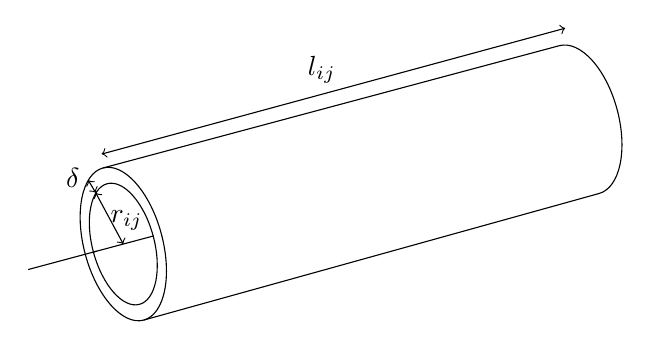
\begin{tikzpicture}[scale=1]
    \begin{scope}[rotate=15]
    \node[transform shape,ellipse,minimum height=2cm,minimum width=1cm,draw,outer sep=0]     (a) {};
    \clip[scale=0.8,postaction={line width=0.8pt,draw}] (a) circle (0.5 and 1);
    \draw[<-](a.west) -- (a.east);
    \end{scope}
    \begin{scope}[rotate=15]
    \draw[] (a.north) --  ++(6,0) arc (90:-90:0.5cm and 1cm-2\pgflinewidth) -- (a.south);
    \draw (a.west) ++(-0.75,0) -- ++(0.9cm,0);
    \node at (-1,0.2) {};
    \draw[<->] (0,0) -- (-0.17,0.72);
    \draw[<->] (-0.17,0.72) -- (-0.22,0.9);
    \node[left] at (-0.2,0.92) {$\delta$};
    \node[right] at (-0.2,0.36) {$r_{ij}$};
    \draw[<->] (0.03,1.175) -- (0.03+0.8+5.3,1.175+0.02);
    \node[above] at (0.03+0.4+2.5,1.175+0.02) {$l_{ij}$};
    \end{scope}
    \end{tikzpicture}
\end{center}


Santa Claus considers the problem that the pipes may get frozen: The longer water flows inside the pipe the more amount of water turns into ice according to the \emph{freezing rule}:

\smallskip
\emph{ The water freezes uniformly along the pipe from the wall to the interior and the thickness of the ice layer is $\tau \alpha$, with $\tau\ge 0$ the duration water that has been running through the pipe and $\alpha > 0$ a constant \textit{freezing rate} (here we neglect the fact that water arrives at the outlet a bit later than at the inlet). Furthermore, when water freezes, its volume expands by 9\%.}

\smallskip
To prevent pipes from getting broken due to that volume expansion, Santa Clause chooses a fixed small positive number $\varepsilon$ first and requires all the pipes to be designed such that their radii are larger than $\varepsilon$. For each pipe $p_{ij}$, the associated water pump engine will stop pumping if the thickness of the ice layer equals $r_{ij} - \varepsilon$ or the water tank of $F_i$ is empty. When a water pump engine stops, we assume that the remaining water between the ice layer flows immediately to the corresponding watermill, and we call that pipe \emph{almost frozen}.

Moreover, to build this network of pipes, there is a fixed amount of steel available which can be used to produce at maximum $M_0$ (in $\rm m^3$) pipe walls.

Santa Claus asks the elves: ``To compute the amount of steel used to build our network, we need to know the total volume of all pipe walls. How can we compute it in terms of the size of the pipes?''

\begin{itemize}
    \item[(i)] \textbf{Amount of necessary steel.} Elf Alice says: ``The total volume of all pipe walls is given by  $\delta\sum_{i=1}^m\sum_{j=1}^n \pi r_{ij}^2l_{ij}$.''
\end{itemize}
Santa Claus continues to ask: ``What can be said when there is no pipe getting almost frozen?''
\begin{itemize}
    \item[(ii)] \textbf{Criterion for almost frozen pipes.} Elf Bob says: ``There is no pipe getting almost frozen if and only if the following inequality holds:
    \begin{align*}
    \frac{r_{ij} - \varepsilon}{\alpha} > t_i\coloneqq\frac{V_i}{\sum_{j=1}^n Q_{ij}} \mbox{ for all } i = 1,\ldots,m,\ j = 1,\ldots,n.\mbox{''}
    \end{align*}
    \item[(iii)] \textbf{Total length estimate.} Elf Camille says: ``The \textit{total length} $l \coloneqq \sum_{i=1}^m\sum_{j=1}^n l_{ij}$ of all pipes in the network satisfies
    \begin{align*}
    l < \frac{M_0}{\pi\delta\left(\delta + 2\varepsilon + 2\alpha\min_{1\le i\le m} t_i\right)}.\mbox{''}
    \end{align*}
    \item[(iv)] \textbf{Length estimate.} Elf Dominic says: ``If the total length of all pipes of each factory are equal, i.e. $\sum_{j=1}^n l_{ij}= l_0$ for all $i$ and a $l_0>0$, then
    \begin{align*}
    l_0 < \frac{M_0}{\pi\delta\left(m\delta + 2m\varepsilon + 2\alpha\sum_{i=1}^m t_i\right)}.\mbox{''}
    \end{align*}
    \item[(v)] \textbf{Capacity estimate.} Elf Elsa says: ``If the total length of all pipes of each factory are equal, the \textit{total capacity} $V$ of all the pipes, defined by
    \begin{align}
    V \coloneqq \sum_{i=1}^m\sum_{j=1}^n \pi r_{ij}^2l_{ij},\label{V}\tag{V}
    \end{align}
    satisfies 
    \begin{align*}
    V > \pi l_0\sum_{i=1}^m (\varepsilon + \alpha t_i)^2.\mbox{''}
    \end{align*}
\end{itemize}
Santa Claus asks again: ``What can be said if there is no water left in any water tank?''
\begin{itemize}
    \item[(vi)] \textbf{Criterion for empty tanks.} Elf Federico says: ``There is no water left in any water tank if and only if
    \begin{align}
    \label{2}
    \tag{${\rm C}_2$}
    \sum_{j=1}^n (r_{ij} - \varepsilon)Q_{ij}\ge\alpha V_i\quad \mbox{ for all } i = 1,\ldots,m.\mbox{''}
    \end{align}    
\end{itemize}
Santa Claus asks: ``In each watermill, bakers will need 10 ${\rm cm}^3$ water to make a cookie. If there is still water in all water tanks after all water pump engines have stopped pumping, how many cookies all watermills can make at maximum?''
\begin{itemize}
    \item[(vii)] \textbf{Amount of cookies.} Elf Gwen says: ``The maximum number of cookies all watermills can produce is given by
    \begin{align*}
    \sum_{i=1}^m\sum_{j=1}^n\left\lfloor 10^5 \left(Q_{ij}\frac{r_{ij} - \varepsilon}{\alpha} - \frac{\pi}{1.09}r_{ij}^2l_{ij}\right)\right\rfloor.\mbox{''}
    \end{align*}
    Here $\lfloor x\rfloor$ is the \textit{integral part} of a real number $x$ which is the largest integer that does not exceed $x$.
\end{itemize}

Which elves are wrong?

\subsection*{Possible answers:}

	% Please give exactly (!) ten possible answers to your challenge!

\begin{enumerate}
    \item None of them
    \item Only Alice
    \item Alice, Camille
    \item Alice, Dominic
    \item Alice, Elsa
    \item Alice, Federico
    \item Alice, Gwen
    \item Alice, Bob, Gwen
    \item Bob, Federico, Dominic
    \item Alice, Camille, Gwen
\end{enumerate}


%\subsection*{Project reference:}

	% Please insert a short description of your project with a reference to the challenge given above!

\newpage%

\subsection{Solution}
\textbf{The right answer is: 7.}\\

% Please give a (detailed) solution to your problem!
(i) \textit{Elf Alice is wrong}. Note that the pipes are cylindrical. The total necessary amount of steel to build all pipes is given by
\begin{align}
M &\coloneqq \sum_{i=1}^m\sum_{j=1}^n \left[\pi(r_{ij} + \delta)^2l_{ij} - \pi r_{ij}^2l_{ij}\right] = \sum_{i=1}^m\sum_{j=1}^n \pi l_{ij}\left(\delta^2 + 2\delta r_{ij}\right).\label{M}\tag{A}
\end{align}
(ii) \textit{Elf Bob is right}. The necessary and sufficient condition in order that there is no pipe getting almost frozen is
\begin{align}
\label{1}
\tag{${\rm C}_1$}
\frac{r_{ij} - \varepsilon}{\alpha} > \frac{V_i}{\sum_{j=1}^n Q_{ij}} \mbox{ for all } i = 1,\ldots,m,\ j = 1,\ldots,n.
\end{align}
Indeed, for each factory $F_i$, the earliest possible time for a pipe to get almost frozen is $t_{i,\min} \coloneqq \min_{1\le j\le n} (r_{ij} - \varepsilon)/\alpha$. The factory $F_i$ pumps water until $t = t_{i,\min}$ if and only if the original amount $V_i$ of water in its water tank is larger than or equal to the amount of water that has been pumped until $t_{i,\min}$, i.e. $V_i\ge t_{i,\min}\sum_{j=1}^n Q_{ij}$. Taking negation, one obtains \eqref{1}.

(iii) \textit{Elf Camille is right}. Due to limited available steel, one has $M\le M_0$. Combining this, \eqref{M}, and \eqref{1} yields
\begin{align*}
M_0&\ge M > \sum_{i=1}^m\sum_{j=1}^n \pi l_{ij}\left(\delta^2 + 2\delta\varepsilon + 2\alpha\delta t_i\right)\\
&\ge\pi\left(\delta^2 + 2\delta\varepsilon + 2\alpha\delta\min_{1\le i\le m} t_i\right)\underbrace{\sum_{i=1}^m\sum_{j=1}^n l_{ij}}_{=:\, l}.
\end{align*}
(iv) \textit{Elf Dominic is right}. As in (ii), combining \eqref{M} and \eqref{1} yields
\begin{align*}
M_0\ge M > \sum_{i=1}^m \pi\left(\delta^2 + 2\delta\varepsilon + 2\alpha\delta t_i\right)\underbrace{\sum_{j=1}^n l_{ij}}_{=:\, l_0}. 
\end{align*}
(v) \textit{Elf Elsa is right}. Similarly, combining \eqref{V} and \eqref{1} yields
\begin{align*}
V > \pi\sum_{i=1}^m (\varepsilon + \alpha t_i)^2\sum_{j=1}^n l_{ij}.
\end{align*}
(vi) \textit{Elf Federico is right}. Indeed, suppose that there is still water in the water tank of a factory $F_i$ for an $i\in \{1,\ldots,m\}$, then all its pipes get almost frozen. The pipe $p_{ij}$ gets almost frozen at the time $t = (r_{ij} - \varepsilon)/\alpha$, hence the volume of water that has been pumped into that pipe is $(r_{ij} - \varepsilon)Q_{ij}/\alpha$. The fact that there is still water in $F_i$ is equivalent to
\begin{align*}
V_i> \sum_{j=1}^n \frac{r_{ij} - \varepsilon}{\alpha}Q_{ij}.
\end{align*}
The opposite direction is obvious. Taking negation, one obtains \eqref{2}. 

(vii) \textit{Elf Gwen is wrong}. Since there is still water in all tanks, all pipes get almost frozen. The amount of water $W_{j}$ receives equals the difference between the amount of water which has been pumped into the pipes and the amount of water getting frozen (not the volume of ice occupying the pipes), and plus the amount of remaining water between the ice layer. Hence, it equals
\begin{align*}
\sum_{i=1}^m \left(Q_{ij}\frac{r_{ij} - \varepsilon}{\alpha} - \frac{\pi}{1.09}(r_{ij}^2 - \varepsilon^2)l_{ij} + \pi\varepsilon^2l_{ij}\right) \mbox{ (in } {\rm m}^3).
\end{align*}
Then the bakers at $W_j$ can make at maximum 
\begin{align*}
\left\lfloor 10^5\sum_{i=1}^m \left(Q_{ij}\frac{r_{ij} - \varepsilon}{\alpha} - \frac{\pi}{1.09}(r_{ij}^2 - \varepsilon^2)l_{ij} + \pi\varepsilon^2l_{ij}\right)\right\rfloor \mbox{ cookies}.
\end{align*}
Thus the maximum number of cookies that can be made in all watermills is
\begin{align*}
\sum_{j=1}^n\left\lfloor 10^5\sum_{i=1}^m \left(Q_{ij}\frac{r_{ij} - \varepsilon}{\alpha} - \frac{\pi}{1.09}(r_{ij}^2 - \varepsilon^2)l_{ij} + \pi\varepsilon^2l_{ij}\right)\right\rfloor.
\end{align*}

\end{document}

%%%%%%%%%%%%%%%%%%%%%%%%%%%%%%%%%%%%%%%%
%%%%%%%%%%%%%%%%%%%%%%%%%%%%%%%%%%%%%%%%


Remarks:

	% State any remarks concerning your challenge here!
	% We try to incorperate your request and ideas concerning the to your challenge.
	% You may also request a date of release.
 

